\documentclass[11pt,a4paper]{article}

\usepackage[margin=1.0in]{geometry}
\usepackage[T1]{fontenc}
\usepackage[utf8]{inputenc}
\usepackage{lmodern}
\usepackage{microtype}
\usepackage{amsmath,amssymb,amsthm,mathtools}
\usepackage{booktabs}
\usepackage{graphicx}
\usepackage{xcolor}
\usepackage{enumitem}
\usepackage{hyperref}
\emergencystretch=2em

\hypersetup{
  colorlinks=true,
  linkcolor=blue!60!black,
  citecolor=green!45!black,
  urlcolor=blue!65!black,
  pdftitle={Quantum Spectral Christoffel-Super-Poincare Inequalities, Exact Piecewise-Logarithmic Mixing Laws, and Machine-Checked Rapid-Mixing Certificates Beyond the Spectral Gap},
  pdfauthor={Lluis Eriksson}
}

\newtheorem{theorem}{Theorem}[section]
\newtheorem{proposition}[theorem]{Proposition}
\newtheorem{lemma}[theorem]{Lemma}
\newtheorem{corollary}[theorem]{Corollary}
\theoremstyle{definition}
\newtheorem{definition}{Definition}[section]
\newtheorem{remark}{Remark}[section]

\newcommand{\R}{\mathbb{R}}
\newcommand{\Q}{\mathbb{Q}}
\newcommand{\C}{\mathbb{C}}
\newcommand{\N}{\mathbb{N}}
\newcommand{\Tr}{\operatorname{Tr}}
\newcommand{\Edir}{\mathcal{E}}
\newcommand{\KMS}{\mathrm{KMS}}
\newcommand{\Kchr}{\mathcal{K}}

\title{\textbf{Quantum Spectral Christoffel--Super-Poincar\'e Inequalities, Exact Piecewise-Logarithmic Mixing Laws, and Machine-Checked Rapid-Mixing Certificates Beyond the Spectral Gap}}

\author{Lluis Eriksson\thanks{Independent researcher (Sweden). Research, zero-dependency Lean~4 proofs, exact-$\Q$ $\mathrm{LDL}^\top$ and convex-hull mixing-time verifiers, and benchmarks prepared with AI assistance (Google Antigravity) and publicly archived at \url{https://github.com/lluiseriksson/beyond-gap-gibbs-certificates}.}}

\date{November 24, 2026}

\begin{document}
\maketitle

\begin{abstract}
Proving rapid mixing of quantum Gibbs samplers beyond high-temperature regimes was recently revolutionized by Chen and Ding~\cite{ChenDing2026BeyondGap}, who established $O(\log^4 n + \log(1/\varepsilon))$ mixing for one-dimensional KMS-detailed-balanced Gibbs samplers by showing that states far from equilibrium carry large weight outside low-weight operator subspaces where stronger dissipation holds. Turning this qualitative mechanism into \emph{exact, non-asymptotic, constant-free} mixing-time certificates for general non-commuting Hamiltonians---without relying on asymptotic hypercontractivity constants and with exact-$\Q$ verification of the quantized spectral-gap and Christoffel bounds---remains open. We resolve this problem with five theorems, a zero-dependency Lean~4 formalization, and an exact-$\Q$ $\mathrm{LDL}^\top$ certificate verifier. First, for any full-rank Gibbs state $\sigma$ and any KMS-symmetric Markov generator with subspace $I \in V \subset \mathcal{B}(\mathcal{H})$ and restricted gap $\lambda(V^\perp)$, we introduce the basis-independent \emph{Quantum Christoffel Operator} $\Kchr_V \coloneqq \sum_{a=1}^D E_a^\dagger E_a$ and prove the exact Quantum Super-Poincar\'e Inequality $\Edir(X_\rho, X_\rho) \ge \lambda(V^\perp)\bigl(\chi^2_\sigma(\rho\|\sigma) - (\|\Kchr_V\|_\infty - 1)\bigr)_+$ for every quantum state $\rho$. Second, for any subspace ladder (Pauli-weight or exact KMS eigenmodes), we integrate the upper convex envelope $\frac{dy}{dt} \le -2\max_k \lambda_k(y - C_k)$ in closed form across exact knots $y_j^* = (\lambda_{k_j} C_{k_j} - \lambda_{k_{j-1}} C_{k_{j-1}})/(\lambda_{k_j} - \lambda_{k_{j-1}})$, proving strict speedup over $T_{\mathrm{gap}}$ whenever $y_0 > y_1^*$ and a universal factor-of-2 optimality law ($T_{\mathrm{SP}}/t_{\mathrm{exact}} \to 1$ as $\varepsilon \to 0^+$ or $y_0 \to \infty$) on 2-tier commuting semigroups. Third, we prove an explicit, constant-free $T_{\mathrm{SP}}(n,\varepsilon) \le \frac{1}{4\gamma}(\log n)^2 + O(\gamma^{-1}(\log n + \log(1/\varepsilon)))$ mixing bound for linear Pauli-weight ladders using pure $L^1 \to L^2$ projection (zero hypercontractivity, with universal $c=3$ for all quantum states and tighter $c=1$ for product-state trajectories under product semigroups), alongside the exact two-regime $\alpha$-Super-Poincar\'e phase diagram across $\alpha \in (0,1)$, $\alpha = 1$, and $\alpha > 1$. Fourth, we lift every convex-hull bound directly to non-asymptotic trace-norm and relative-entropy decay $D(\rho_t\|\sigma) \le D_2(\rho_t\|\sigma) \le \log(1 + y_{\mathrm{env}}(t))$. Fifth, we construct cryptographically linked global operator-order exact-$\Q$ $\mathrm{LDL}^\top$ PSD witnesses certifying both subspace gaps and Christoffel norms strictly over $\Q$ on the quantized operator bundle given perturbation radii $\delta_*^{\Q}$ (with our synthesis script estimating $\delta_*^{\Q}$ against double-precision \texttt{eigh(H)} for interacting chains, while analytical depolarizing certificates are end-to-end exact-$\Q$ with zero floating-point input). All 16 core algebraic theorems are formalized in Lean~4 (\texttt{v4.35.0}, 0 \texttt{sorry}, 0 \texttt{Classical.choice}) and benchmarked on non-commuting 1D tilted/ferromagnetic TFIM ($1.26\times$--$3.30\times$ speedup for $n=3, 4$; $1.65\times$--$3.30\times$ at $n=4$) and XXZ ($1.57\times$) KMS Gibbs samplers, $n = 10$--$1{,}000$ depolarizing chains ($17.7\times$ universal $c=3$ and $20.7\times$ product-state $c=1$ speedup), and 6 exact-$\Q$ certificates containing 14 verified linked $\mathrm{LDL}^\top$ PSD witnesses.
\end{abstract}

\section{Introduction}
\label{sec:intro}

Preparing thermal Gibbs states $\sigma = e^{-\beta H}/\Tr(e^{-\beta H})$ of interacting quantum spin systems via dissipative Lindbladian evolution is a central primitive of quantum simulation and quantum statistical mechanics~\cite{Davies1979Generators,ChenKastoryanoGilyen2023,BardetCapelGaoLuciaPerezGarciaRouze2023}. Traditional convergence bounds rely on the Poincaré spectral gap $\mu_1$ of the Kubo--Martin--Schwinger (KMS)-symmetric Lindbladian $\mathcal{L}^\dagger$, yielding the worst-case mixing time $T_{\mathrm{gap}}(\varepsilon) = \frac{1}{2\mu_1}\log\bigl(\chi^2_\sigma(\rho_0\|\sigma)/\varepsilon^2\bigr) = O(n + \log(1/\varepsilon))$~\cite{Temme2010Chi2} because $\chi^2_\sigma(\rho_0\|\sigma) \le \lambda_{\min}(\sigma)^{-1} - 1$ grows exponentially in system size $n$. Overcoming this linear-$n$ bottleneck typically required proving a uniform quantum Modified Logarithmic Sobolev Inequality (MLSI)~\cite{KastoryanoTemme2013QMLSI}, which had remained open for non-commuting spin chains at arbitrary inverse temperature $\beta > 0$.

In a major recent breakthrough, Chen and Ding~\cite{ChenDing2026BeyondGap} proved rapid mixing $O(\log^4 n + \log(1/\varepsilon))$ for one-dimensional non-commuting KMS quantum Gibbs samplers at every positive temperature via \emph{spectral analysis beyond the spectral gap}: any state far from $\sigma$ must carry significant $\chi^2_\sigma$ weight outside the span of low-weight Pauli operators, where higher-weight dissipation rates drive a rapid initial (double-exponential) burn-in before the spectral gap $\mu_1$ governs the final exponential tail.

To convert this paradigm into an exact, assumption-light, finite-size certification engine---analogous to classical Super-Poincar\'e theory~\cite{Wang2000Functional,BakryGentilLedoux2014} and complementing our recent machine-checked spectral certificates~\cite{Antigravity2026Purity,Antigravity2026Continuum}---three questions arise:
\begin{enumerate}[leftmargin=1.6em,itemsep=2pt]
  \item \textbf{Exact Non-Commuting Projection Geometry:} What is the sharpest basis-independent operator invariant controlling the $\KMS$ $L^1(\sigma) \to L^2(\sigma)$ projection norm on a subspace $V \subset \mathcal{B}(\mathcal{H})$?
  \item \textbf{Closed-Form Mixing Law \& Sharpness:} Given a discrete ladder of subspace gaps and projection norms $\{(\lambda_k, \overline{\Lambda}_k)\}_{k=0}^m$, what is the exact closed-form mixing time, how tight is it against true semigroup trajectories, and what scaling does pure $L^1 \to L^2$ projection achieve without hypercontractivity?
  \item \textbf{Zero-Floating-Point-Trust Certification:} Can both the higher-tier spectral gaps $\lambda_k$, the Christoffel norms $\overline{\Lambda}_k$, and the resulting mixing time $T_{\mathrm{SP}}(\varepsilon)$ be certified strictly in exact rational arithmetic $\Q$ with machine-checked Lean~4 soundness?
\end{enumerate}

We answer all three questions completely in Sections~\ref{sec:christoffel}--\ref{sec:experiments}.

\section{Quantum Spectral Christoffel--Super-Poincar\'e Inequalities}
\label{sec:christoffel}

Let $\mathcal{H}$ be a finite-dimensional Hilbert space ($d = \dim\mathcal{H}$) and $\sigma \succ 0$ ($\Tr\sigma = 1$) a full-rank Gibbs state. Equip $\mathcal{B}(\mathcal{H})$ with the KMS inner product and norm
\begin{equation}
  \langle X, Y \rangle_{\KMS} \;\coloneqq\; \Tr\!\bigl(\sigma^{1/2} X^\dagger \sigma^{1/2} Y\bigr), \qquad
  \|X\|_{2,\sigma}^2 \;\coloneqq\; \langle X, X \rangle_{\KMS}.
  \label{eq:kms_ip}
\end{equation}
For any quantum state $\rho \succeq 0$ ($\Tr\rho = 1$), its KMS relative density $X_\rho \coloneqq \sigma^{-1/2}\rho\sigma^{-1/2} \succeq 0$ satisfies $\langle I, X_\rho \rangle_{\KMS} = \Tr\rho = 1$, $\|X_\rho\|_{2,\sigma}^2 = \Tr\bigl((\sigma^{-1/4}\rho\sigma^{-1/4})^2\bigr) = e^{D_2(\rho\|\sigma)}$ (where $D_2$ is the sandwiched R\'enyi-2 divergence~\cite{MullerLennert2013Sandwiched}), and
\begin{equation}
  \chi^2_\sigma(\rho\|\sigma) \;\coloneqq\; \|X_\rho - I\|_{2,\sigma}^2 \;=\; e^{D_2(\rho\|\sigma)} - 1.
  \label{eq:chi2_def}
\end{equation}
Moreover, setting $B \coloneqq \sigma^{1/4}(X_\rho - I)\sigma^{1/4} = \sigma^{-1/4}(\rho - \sigma)\sigma^{-1/4}$, matrix H\"older's inequality ($\|UVW\|_1 \le \|U\|_4\|V\|_2\|W\|_4$) gives the exact constant-1 trace-norm domination
\begin{equation}
  \|\rho - \sigma\|_1 \;=\; \|\sigma^{1/4} B \sigma^{1/4}\|_1 \;\le\; (\Tr\sigma)^{1/4}\|B\|_2 (\Tr\sigma)^{1/4} \;=\; \sqrt{\chi^2_\sigma(\rho\|\sigma)}
  \label{eq:trace_chi2}
\end{equation}
(discrete weighted form proved in Lean~4: \texttt{trace\_norm\_sq\_le\_chi2}).

Let $\mathcal{L}^\dagger$ be a Heisenberg-picture Lindbladian that is KMS-symmetric ($\langle X, \mathcal{L}^\dagger Y \rangle_{\KMS} = \langle \mathcal{L}^\dagger X, Y \rangle_{\KMS}$) and primitive ($\ker\mathcal{L}^\dagger = \C I$), with nonnegative Dirichlet form $\Edir(X, X) \coloneqq \langle X, (-\mathcal{L}^\dagger) X \rangle_{\KMS} \ge 0$. Under $\rho_t = e^{t\mathcal{L}}(\rho_0)$, $X_{\rho_t} = e^{t\mathcal{L}^\dagger}(X_{\rho_0})$ obeys $\frac{d}{dt}\chi^2_\sigma(\rho_t\|\sigma) = -2\Edir(X_{\rho_t}, X_{\rho_t})$.

\subsection{Basis-Independent Quantum Christoffel Operator and Super-Poincar\'e Bound}

\begin{definition}[Quantum Christoffel Operator]
\label{def:christoffel}
Let $V \subset \mathcal{B}(\mathcal{H})$ be any subspace containing $I$, and let $\{E_1, \dots, E_D\}$ be any $\KMS$-orthonormal basis of $V$ ($\langle E_a, E_b \rangle_{\KMS} = \delta_{ab}$). The \emph{Quantum Christoffel Operator} of $V$ is
\[
  \Kchr_V \;\coloneqq\; \sum_{a=1}^D E_a^\dagger E_a \;\succeq\; I,
  \qquad
  \overline{\Lambda}_V \;\coloneqq\; \|\Kchr_V\|_\infty,
  \qquad
  \Lambda_V \;\coloneqq\; \sup_{\|\psi\|=1} \sum_{a=1}^D \bigl|\langle \psi | E_a | \psi \rangle\bigr|^2.
\]
\end{definition}

Note that $\Kchr_V$ is strictly invariant under any unitary change of $\KMS$-orthonormal basis $E'_a = \sum_b U_{ab} E_b$ (since $U^\dagger U = I_D$), and when $\sigma = I/2^n$ with $V = \operatorname{span}\{P : |P| \le k\}$, $\Kchr_V = \bigl(\sum_{j=0}^k \binom{n}{j} 3^j\bigr) I$.

\begin{theorem}[Quantum Spectral Christoffel--Super-Poincar\'e Inequality]
\label{thm:christoffel_sp}
Let $I \in V \subset \mathcal{B}(\mathcal{H})$ have $\KMS$-orthogonal projection $P_V$, and define its \emph{operator-order dissipation constant}
\[
  \lambda_{\mathrm{op}}(V^\perp) \;\coloneqq\;
  \sup\bigl\{\lambda \ge 0 : -\mathcal{L}^\dagger \succeq \lambda(I - P_V) \text{ in } L^2(\KMS)\bigr\}
  \;=\; \inf_{X \notin V} \frac{\Edir(X, X)}{\|(I - P_V) X\|_{2,\sigma}^2}.
\]
Then for \emph{every} quantum state $\rho$:
\begin{enumerate}[label=(\alph*),leftmargin=2em,itemsep=2pt]
  \item $1 \le \Lambda_V \le \overline{\Lambda}_V$, and the centered projection satisfies $\|P_V(X_\rho - I)\|_{2,\sigma}^2 \le \Lambda_V - 1 \le \overline{\Lambda}_V - 1$ (see Table~\ref{tab:lean_manifest}).
  \item The Dirichlet form obeys the exact Quantum Super-Poincar\'e Inequality (Table~\ref{tab:lean_manifest}):
  \begin{equation}
    \Edir(X_\rho, X_\rho) \;\ge\; \lambda_{\mathrm{op}}(V^\perp)\,\Bigl(\chi^2_\sigma(\rho\|\sigma) - (\overline{\Lambda}_V - 1)\Bigr)_+.
    \label{eq:single_sp}
  \end{equation}
  In particular, writing $V = \C I \oplus V_+$, $\lambda_{\mathrm{op}}(V^\perp) = \lambda_{\min}\bigl(M_{\perp\perp} - M_{\perp V_+} M_{V_+ V_+}^{-1} M_{V_+ \perp}\bigr)$ is the exact Schur complement, coinciding identically with the $(r+1)$-th eigenvalue $\mu_{r+1}$ on every $\mathcal{L}^\dagger$-invariant eigenmode subspace $V_r = \operatorname{span}\{E_0, \dots, E_r\}$.
  \item For any subspace filtration $I \in V_0 \subset V_1 \subset \dots \subset V_m$ with $C_k \coloneqq \overline{\Lambda}_{V_k} - 1$ and $\lambda_k \coloneqq \lambda_{\mathrm{op}}(V_k^\perp)$, the piecewise-linear convex envelope satisfies (Lean: \texttt{super\_poincare\_envelope\_two})
  \begin{equation}
    \Edir(X_\rho, X_\rho) \;\ge\; \Phi_{\mathrm{env}}\bigl(\chi^2_\sigma(\rho\|\sigma)\bigr)
    \;\coloneqq\; \max_{0 \le k \le m} \lambda_k \bigl(\chi^2_\sigma(\rho\|\sigma) - C_k\bigr).
    \label{eq:envelope_sp}
  \end{equation}
\end{enumerate}
\end{theorem}

\begin{proof}
For any state $\rho$, $\langle E_a, X_\rho \rangle_{\KMS} = \Tr(\sigma^{1/2} E_a^\dagger \sigma^{1/2} \sigma^{-1/2}\rho\sigma^{-1/2}) = \Tr(E_a^\dagger \rho)$, hence $\|P_V X_\rho\|_{2,\sigma}^2 = \sum_{a=1}^D |\Tr(E_a^\dagger \rho)|^2$. Because $\rho \mapsto |\Tr(E_a^\dagger \rho)|^2$ is convex on the compact convex state space, the maximum of the sum is attained at an extreme point $\rho = |\psi\rangle\langle\psi|$ ($\|\psi\| = 1$), giving $\|P_V X_\rho\|_{2,\sigma}^2 \le \Lambda_V$. By Cauchy--Schwarz, $|\langle \psi | E_a | \psi \rangle|^2 \le \|E_a |\psi\rangle\|^2 = \langle \psi | E_a^\dagger E_a | \psi \rangle$; summing over $a = 1, \dots, D$ yields $\Lambda_V \le \sup_{\|\psi\|=1} \langle \psi | \Kchr_V | \psi \rangle = \overline{\Lambda}_V$. Since $I \in V$ and $\langle I, X_\rho - I \rangle_{\KMS} = 0$, orthogonality gives $\|P_V X_\rho\|_{2,\sigma}^2 = 1 + \|P_V(X_\rho - I)\|_{2,\sigma}^2$, proving (a). For (b), by definition of $\lambda_{\mathrm{op}}(V^\perp)$,
\[
  \Edir(X_\rho, X_\rho) \;=\; \Edir(X_\rho - I, X_\rho - I)
  \;\ge\; \lambda_{\mathrm{op}}(V^\perp)\,\|(I - P_V)(X_\rho - I)\|_{2,\sigma}^2.
\]
Pythagoras yields $\|(I - P_V)(X_\rho - I)\|_{2,\sigma}^2 = \chi^2_\sigma(\rho\|\sigma) - \|P_V(X_\rho - I)\|_{2,\sigma}^2 \ge \chi^2_\sigma(\rho\|\sigma) - (\overline{\Lambda}_V - 1)$, proving~\eqref{eq:single_sp} and~\eqref{eq:envelope_sp}. The Schur-complement formula follows from block positivity of $M_{\KMS} - \lambda(I - P_V)$ on $(\C I)^\perp = V_+ \oplus V^\perp$ (where $M_{V_+ V_+} \succ 0$ by primitivity), reducing to $M_{\perp\perp} \succeq \mu_{r+1} I_\perp$ whenever $M_{\perp V_+} = 0$.
\end{proof}

\subsection{Exact Upper-Convex-Hull Piecewise-Logarithmic Mixing Law and Sharpness}

\begin{theorem}[Exact Piecewise-Logarithmic Mixing Law and 2-Tier Optimality]
\label{thm:hull_mixing}
Let $\{(\lambda_{k_j}, C_{k_j})\}_{j=0}^r$ ($0 < \lambda_{k_0} < \dots < \lambda_{k_r}$, $0 = C_{k_0} < \dots < C_{k_r}$) be the minimal active upper convex hull of the affine functions $\ell_k(y) = \lambda_k(y - C_k)$ on $(0, \infty)$ satisfying~\eqref{eq:envelope_sp}, with transition knots $y_0^* = 0$, $y_{r+1}^* = +\infty$, and $y_j^* = (\lambda_{k_j} C_{k_j} - \lambda_{k_{j-1}} C_{k_{j-1}})/(\lambda_{k_j} - \lambda_{k_{j-1}})$ ($1 \le j \le r$). Then:
\begin{enumerate}[label=(\alph*),leftmargin=2em,itemsep=2pt]
  \item \textbf{Well-Posedness and Exact Mixing Time.} The knots satisfy $0 < y_1^* < \dots < y_r^*$ and $y_j^* > C_{k_j}$ for all $j \ge 1$ (Table~\ref{tab:lean_manifest}). For every initial state $\rho_0$ with $y_0 = \chi^2_\sigma(\rho_0\|\sigma) > \varepsilon^2 > 0$, the exact piecewise-linear envelope solution $y_{\mathrm{env}}(t)$ satisfies $\chi^2_\sigma(\rho_t\|\sigma) \le y_{\mathrm{env}}(t)$ for all $t \ge 0$, and hence $\|\rho_t - \sigma\|_1 \le \varepsilon$ for all
  \begin{equation}
    t \;\ge\; T_{\mathrm{SP}}(\varepsilon; y_0) \;\coloneqq\;
    \sum_{j=0}^{r} \frac{1}{2\lambda_{k_j}}
    \log\!\left(\frac{\min(y_0, y_{j+1}^*) - C_{k_j}}{\max(\varepsilon^2, y_j^*) - C_{k_j}}\right)
    \mathbf{1}_{\min(y_0, y_{j+1}^*) > \max(\varepsilon^2, y_j^*)}.
    \label{eq:T_sp_exact}
  \end{equation}
  \item \textbf{Strict Speedup over Spectral Gap.} Whenever $y_0 > y_1^*$ and $\lambda_{k_1} > \lambda_{k_0}$, we have $T_{\mathrm{SP}}(\varepsilon; y_0) < T_{\mathrm{gap}}(\varepsilon; y_0) \coloneqq \frac{1}{2\lambda_{k_0}}\log(y_0/\varepsilon^2)$ strictly (Table~\ref{tab:lean_manifest}).
  \item \textbf{Universal Factor-of-2 Sharpness on 2-Tier Semigroups.} For any $0 < \lambda_0 < \lambda_1$ and $C_1 > \varepsilon^2$, consider the 2-tier commuting semigroup with $\chi^2(t) = C_1 e^{-2\lambda_0 t} + (y_0 - C_1) e^{-2\lambda_1 t}$ ($y_0 > y_1^*$) and exact $\chi^2$-hitting time $t_{\mathrm{exact}}(\varepsilon)$. Then
  \begin{equation}
    t_{\mathrm{exact}}(\varepsilon) \;\le\; T_{\mathrm{SP}}(\varepsilon; y_0)
    \;\le\; 2\, t_{\mathrm{exact}}(\varepsilon)
    + \frac{1}{2\lambda_0}\log\frac{\lambda_1}{\lambda_1 - \lambda_0}
    + \frac{1}{2\lambda_1}\log_+\!\left(\frac{\lambda_1 - \lambda_0}{\lambda_0}\right),
    \label{eq:sharp_2tier}
  \end{equation}
  and $T_{\mathrm{SP}}(\varepsilon; y_0) / t_{\mathrm{exact}}(\varepsilon) \to 1$ in both asymptotic regimes $\varepsilon \to 0^+$ (fixed $y_0$) and $y_0 \to \infty$ (fixed $\varepsilon$).
\end{enumerate}
\end{theorem}

\begin{proof}
Because $\Phi_{\mathrm{env}}(y)$ is continuous, strictly increasing, and piecewise linear on $(0, \infty)$ with active slope $\lambda_{k_j}$ and intercept $-\lambda_{k_j} C_{k_j}$ on $[y_j^*, y_{j+1}^*]$ (Lean: \texttt{hull\_tier2\_dominates\_above}, \texttt{hull\_tier1\_dominates\_below}), comparison of $\frac{dy}{dt} \le -2\Phi_{\mathrm{env}}(y)$ gives $\chi^2_\sigma(\rho_t\|\sigma) \le y_{\mathrm{env}}(t)$, where the time required for $y_{\mathrm{env}}$ to descend from $y_0$ to $\varepsilon^2$ is $\int_{\varepsilon^2}^{y_0} \frac{dy}{2\Phi_{\mathrm{env}}(y)}$, which evaluates term-by-term to~\eqref{eq:T_sp_exact}. Part (b) follows immediately from $\frac{1}{2\Phi_{\mathrm{env}}(y)} < \frac{1}{2\lambda_{k_0} y}$ on $(y_1^*, y_0]$. For (c), $t_{\mathrm{exact}} \le T_{\mathrm{SP}}$ holds by (a). Since $C_1 e^{-2\lambda_0 t_{\mathrm{exact}}} \le \varepsilon^2$ and $(y_0 - C_1) e^{-2\lambda_1 t_{\mathrm{exact}}} \le \varepsilon^2$, we have $t_{\mathrm{exact}} \ge \max\bigl(\frac{1}{2\lambda_0}\log\frac{C_1}{\varepsilon^2},\; \frac{1}{2\lambda_1}\log\frac{y_0 - C_1}{\varepsilon^2}\bigr)$. Writing $y_1^* = \frac{\lambda_1}{\lambda_1 - \lambda_0} C_1$ and $y_1^* - C_1 = \frac{\lambda_0}{\lambda_1 - \lambda_0} C_1$,
\begin{align*}
  T_{\mathrm{SP}}(\varepsilon; y_0)
  &= \frac{1}{2\lambda_0}\log\frac{C_1}{\varepsilon^2} + \frac{1}{2\lambda_0}\log\frac{\lambda_1}{\lambda_1 - \lambda_0}
   + \frac{1}{2\lambda_1}\log\frac{y_0 - C_1}{\varepsilon^2} + \frac{1}{2\lambda_1}\log\frac{\varepsilon^2}{y_1^* - C_1} \\
  &\le 2\,t_{\mathrm{exact}}(\varepsilon) + \frac{1}{2\lambda_0}\log\frac{\lambda_1}{\lambda_1 - \lambda_0} + \frac{1}{2\lambda_1}\log_+\!\left(\frac{\lambda_1 - \lambda_0}{\lambda_0}\right),
\end{align*}
using $\varepsilon^2 < C_1$ in the last step. When $\varepsilon \to 0^+$ (fixed $y_0$), the first term dominates both $t_{\mathrm{exact}}$ and $T_{\mathrm{SP}}$; when $y_0 \to \infty$ (fixed $\varepsilon$), the third term dominates both, yielding $T_{\mathrm{SP}}/t_{\mathrm{exact}} \to 1$ in either limit.
\end{proof}

\section{Pure \texorpdfstring{$L^1 \to L^2$}{L1 -> L2} Poly-Logarithmic Speedup and Two-Regime Phase Diagram}
\label{sec:scaling}

\begin{theorem}[Pure $L^1 \to L^2$ $(\log n)^2$ Scaling and $\alpha$-Phase Diagram]
\label{thm:scaling_phases}
\begin{enumerate}[label=(\alph*),leftmargin=2em,itemsep=2pt]
  \item \textbf{Constant-Free $O(\log^2 n)$ Bound Without Hypercontractivity.} Suppose an $n$-qubit ($n \ge 2$) KMS-symmetric semigroup with $y_0 = 2^n - 1$ satisfies~\eqref{eq:envelope_sp} along a trajectory $\rho_t$ with linear Pauli-weight dissipation $\lambda_k \ge \gamma(k + 1)$ ($\gamma > 0$) and Christoffel bounds $C_k \le \sum_{j=0}^k \binom{n}{j} c^j - 1$ ($c \ge 1$). Specifically: (i)~$c = 3$ holds \emph{universally for every (possibly entangled) quantum state $\rho$} via Definition~\ref{def:christoffel} ($\Kchr_{V_k} = \bigl(\sum_{j=0}^k \binom{n}{j} 3^j\bigr) I$); and (ii)~$c = 1$ holds \emph{for every product-state trajectory} $\rho_t = \bigotimes_{i=1}^n \rho_{i,t}$ (which is invariant under product/local depolarizing semigroups), because each single-qubit Bloch vector satisfies $\langle X_i\rangle^2 + \langle Y_i\rangle^2 + \langle Z_i\rangle^2 \le 1$ and multiplicativity yields $\sum_{|P|=j} |\Tr(P\rho_t)|^2 = \sum_{|S|=j}\prod_{i \in S}(\langle X_i\rangle^2 + \langle Y_i\rangle^2 + \langle Z_i\rangle^2) \le \binom{n}{j}$ (whereas general entangled states can exceed $c=1$, e.g.\ the 5-qubit $\llbracket 5,1,3\rrbracket$ code state has weight-4 sector sum $S_4 = 15 > \binom{5}{4} = 5$, requiring the universal $c=3$ bound). Then for every $\varepsilon \in (0, 1)$,
  \begin{equation}
    T_{\mathrm{SP}}(\varepsilon; y_0) \;\le\;
    \frac{1}{4\gamma}(\log n)^2 + \frac{1 + \log(2(c + 1))}{2\gamma}\log n + \frac{\log(2 c / \varepsilon^2)}{2\gamma},
    \label{eq:log2n_bound}
  \end{equation}
  an exponential $O(n/\log^2 n)$ speedup over $T_{\mathrm{gap}}(\varepsilon; y_0) = \frac{1}{2\gamma}\log\bigl((2^n - 1)/\varepsilon^2\bigr) = \Theta(n/\gamma)$ without invoking hypercontractivity.
  \item \textbf{Two-Regime $\alpha$-Super-Poincar\'e Phase Diagram.} Suppose a bounded KMS-symmetric semigroup has spectral gap $\mu_1 > 0$ (so $\Edir(X_\rho, X_\rho) \ge \mu_1 y$ for all $y \ge 0$) and additionally satisfies the burn-in Super-Poincar\'e bound $\Edir(X_\rho, X_\rho) \ge \gamma(1 + y)\bigl(\log(1 + y)\bigr)^\alpha$ ($\gamma > 0, \alpha > 0$) whenever $D_2(\rho\|\sigma) \coloneqq \log(1 + y) \ge 1$. Then during the burn-in stage ($D_2(t) \ge 1$), $\frac{d}{dt}D_2(t) \le -2\gamma D_2(t)^\alpha$ integrates in closed form, and pairing with $\mu_1 > 0$ below $D_2 = 1$ yields three exact non-vacuous regimes:
  \begin{itemize}[leftmargin=1.5em,itemsep=1pt]
    \item \emph{Sub-logarithmic ($\alpha \in (0, 1)$):} $D_2(t)^{1-\alpha} \le D_2(0)^{1-\alpha} - 2\gamma(1-\alpha)t$ while $D_2(t) \ge 1$, reaching $D_2 = 1$ in time $\le \frac{D_2(0)^{1-\alpha} - 1}{2\gamma(1-\alpha)}$, hence $T_{\mathrm{mix}}(\varepsilon) = O\bigl(\gamma^{-1} D_2(0)^{1-\alpha} + \mu_1^{-1}\log(1/\varepsilon)\bigr)$.
    \item \emph{Quantum R\'enyi-2 LSI ($\alpha = 1$):} $D_2(t) \le e^{-2\gamma t} D_2(0)$ while $D_2(t) \ge 1$ (and globally if the bound holds on all $y \ge 0$), yielding $T_{\mathrm{mix}}(\varepsilon) \le \frac{1}{2\gamma}\log_+ D_2(0) + \frac{1}{2\mu_1}\log\bigl((e - 1)/\varepsilon^2\bigr) = O(\log n + \log(1/\varepsilon))$.
    \item \emph{Ultracontractive ($\alpha > 1$):} $D_2(t) \le \bigl(D_2(0)^{-(\alpha-1)} + 2\gamma(\alpha - 1)t\bigr)^{-1/(\alpha-1)} \le \bigl(2\gamma(\alpha - 1)t\bigr)^{-1/(\alpha-1)}$ while $D_2(t) \ge 1$, giving uniform $y_0$-independent burn-in down to $D_2 = 1$ in time $\le \bigl(2\gamma(\alpha - 1)\bigr)^{-1}$ followed by exponential tail decay $\frac{1}{2\mu_1}\log\bigl((e - 1)/\varepsilon^2\bigr)$.
  \end{itemize}
\end{enumerate}
\end{theorem}

\begin{proof}
For (a), let $B_k \coloneqq \sum_{j=0}^k \binom{n}{j} c^j - 1 \ge C_k$, and let $m \ge 1$ be the largest integer with $2 B_m \le y_0$ (if $y_0 < 2 B_1 = 2cn$, tier $k = 0$ alone gives $T_{\mathrm{SP}} \le \frac{1}{2\gamma}\log(2cn/\varepsilon^2)$, satisfying~\eqref{eq:log2n_bound}). Partition $[\varepsilon^2, y_0]$ at the split points $z_k = 2 B_k$ ($1 \le k \le m$), $z_{m+1} = y_0$. Since $\Phi_{\mathrm{env}}(y) \ge \gamma(k+1)(y - B_k)$ on $[z_k, z_{k+1}]$,
\[
  T_{\mathrm{SP}}(\varepsilon; y_0) \;\le\; \frac{1}{2\gamma}\log\frac{2 B_1}{\varepsilon^2}
  + \sum_{k=1}^{m} \frac{1}{2\gamma(k+1)}\log\frac{z_{k+1} - B_k}{z_k - B_k}.
\]
Because $z_k - B_k = B_k$ and $z_{k+1} - B_k < 2 B_{k+1}$ (holding also at $k = m$ since $y_0 < 2 B_{m+1}$), and $\frac{B_{k+1}}{B_k} = 1 + \frac{\binom{n}{k+1} c^{k+1}}{B_k} \le 1 + \frac{c(n - k)}{k + 1} \le \frac{(c + 1)n}{k + 1}$ (using $B_k \ge \binom{n}{k} c^k$ for $k \ge 1$), every summand satisfies $\frac{z_{k+1} - B_k}{z_k - B_k} \le \frac{2(c+1)n}{k+1}$. Since $x \mapsto \frac{1}{x}\log\frac{2(c+1)n}{x}$ is decreasing on $[1, n]$ and $m + 1 \le n$, integral comparison gives
\[
  \sum_{k=1}^{m} \frac{1}{2\gamma(k+1)}\log\frac{2(c+1)n}{k+1}
  \;\le\; \frac{1}{2\gamma}\int_1^n \frac{\log(2(c+1)n/x)}{x}\,dx
  \;=\; \frac{1}{4\gamma}(\log n)^2 + \frac{\log(2(c+1))}{2\gamma}\log n.
\]
Adding $\frac{1}{2\gamma}\log\frac{2 c n}{\varepsilon^2}$ yields~\eqref{eq:log2n_bound}. Part (b) follows directly from $\frac{d}{dt}\log(1 + y) = -\frac{2}{1+y}\Edir(X_{\rho_t}, X_{\rho_t}) \le -2\gamma(\log(1+y))^\alpha$ and exact separation of variables.
\end{proof}

\section{Two-Stage Relative-Entropy Contraction and Exact-\texorpdfstring{$\Q$}{Q} \texorpdfstring{$\mathrm{LDL}^\top$}{LDLT} Certificates}
\label{sec:certificates}

\begin{theorem}[Non-Asymptotic Relative-Entropy and R\'enyi-2 Dissipation Lift]
\label{thm:entropy_lift}
Under the hypotheses of Theorem~\ref{thm:hull_mixing}, every certified convex-hull envelope $y_{\mathrm{env}}(t)$ simultaneously certifies, for all $t \ge 0$,
\begin{equation}
  \|\rho_t - \sigma\|_1 \;\le\; \sqrt{y_{\mathrm{env}}(t)}, \qquad
  D(\rho_t\|\sigma) \;\le\; D_2(\rho_t\|\sigma) \;\le\; \log\bigl(1 + y_{\mathrm{env}}(t)\bigr).
  \label{eq:entropy_lift}
\end{equation}
Moreover, whenever $y(t) \ge \max(1, 2 C_k)$, tier $k$ drives linear decay of the sandwiched R\'enyi-2 divergence at rate at least $\lambda_k / 2$: $\frac{d}{dt} D_2(\rho_t\|\sigma) \le -\frac{2\lambda_k(y - C_k)}{1 + y} \le -\frac{1}{2}\lambda_k$.
\end{theorem}

\begin{proof}
Monotonicity of sandwiched R\'enyi divergences in order $\alpha \in [1, 2]$~\cite{MullerLennert2013Sandwiched} gives $D(\rho_t\|\sigma) \le D_2(\rho_t\|\sigma) = \log(1 + \chi^2_\sigma(\rho_t\|\sigma)) \le \log(1 + y_{\mathrm{env}}(t))$, while~\eqref{eq:trace_chi2} yields $\|\rho_t - \sigma\|_1 \le \sqrt{y_{\mathrm{env}}(t)}$. For $y \ge \max(1, 2 C_k)$, $y - C_k \ge y/2$ and $y/(1 + y) \ge 1/2$, so $\frac{d}{dt}D_2 = -\frac{2}{1+y}\Edir \le -\frac{2\lambda_k(y/2)}{1+y} \le -\frac{1}{2}\lambda_k$.
\end{proof}

To eliminate floating-point eigensolver trust completely, we certify both the subspace gaps $\lambda_k$ and the Christoffel norms $\overline{\Lambda}_k$ strictly over $\Q$ via exact rational $\mathrm{LDL}^\top$ factorizations (without square roots!).

\begin{theorem}[Zero-Floating-Point-Trust Global Operator-Order $\mathrm{LDL}^\top$ Certificate]
\label{thm:ldlt_cert}
Let $M_{\KMS} = -\Gamma_\sigma^{1/2}\mathcal{L}^\dagger\Gamma_\sigma^{-1/2} \in \R^{d^2 \times d^2}$ be the real-symmetric KMS generator matrix (for real-symmetric $H$ and jumps), let $P_0 = |B_0\rangle\langle B_0|$ be the 1D stationary projector ($M_{\KMS} B_0 = 0$), let $V_k \ni I$ be \emph{any} subspace (not required to be $\mathcal{L}^\dagger$-invariant) with $\KMS$-orthogonal projector $P_{V_k}$, and let $\tilde{M}, \tilde{P}_0, \tilde{P}_k \in \Q^{d^2 \times d^2}$ and $\tilde{\Kchr}_k \in \Q^{d \times d}$ satisfy certified Frobenius bounds $\|\tilde{M} - M_{\KMS}\|_F \le \delta_M^{\Q}$, $\|\tilde{P}_0 - P_0\|_F \le \delta_{P_0}^{\Q}$, $\|\tilde{P}_k - P_{V_k}\|_F \le \delta_P^{\Q}$, and $\|\tilde{\Kchr}_k - \Kchr_{V_k}\|_F \le \delta_K^{\Q}$ with $\delta_M^{\Q}, \delta_{P_0}^{\Q}, \delta_P^{\Q}, \delta_K^{\Q} \ge 0$ and $\lambda_k^{\Q} > 0$, $\beta_0 > 0$. Suppose exact rational unit lower-triangular matrices $L_1, L_2$ and nonnegative rational diagonals $D_1, D_2 \ge 0$ satisfy:
\begin{enumerate}[label=(\roman*),leftmargin=2em,itemsep=2pt]
  \item $\tilde{M} + \beta_0 \tilde{P}_0 + \lambda_k^{\Q} \tilde{P}_k - (\lambda_k^{\Q} + \delta_M^{\Q} + \beta_0 \delta_{P_0}^{\Q} + \lambda_k^{\Q} \delta_P^{\Q}) I \;=\; L_1 \operatorname{diag}(D_1) L_1^\top$, and
  \item $(\overline{\Lambda}_k^{\Q} - \delta_K^{\Q}) I - \tilde{\Kchr}_k \;=\; L_2 \operatorname{diag}(D_2) L_2^\top$.
\end{enumerate}
Then $\lambda_{\mathrm{op}}(V_k^\perp) \ge \lambda_k^{\Q}$ and $\|\Kchr_{V_k}\|_\infty \le \overline{\Lambda}_k^{\Q}$ hold globally over $\C^{d^2}$ with mathematical certainty (verified in Lean~4; Table~\ref{tab:lean_manifest}), and evaluating~\eqref{eq:T_sp_exact} with the exact unquantized rational logarithm upper bound $\mathrm{log}_{\Q}^{\mathrm{ub,exact}}$ certifies $T_{\mathrm{SP}}(\varepsilon; y_0) \le T_{\mathrm{SP}}^{\Q}$ strictly over $\Q$.
\end{theorem}

\begin{proof}
Because $A \in \R^{m \times m}$ is real symmetric, $A = L \operatorname{diag}(D) L^\top$ with $D \ge 0$ implies $v^\dagger A v = \operatorname{Re}(v)^\top A \operatorname{Re}(v) + \operatorname{Im}(v)^\top A \operatorname{Im}(v) \ge 0$ for all $v \in \C^m$ (\texttt{ldlt\_quad\_nonneg}). By (i), $\tilde{M} + \beta_0 \tilde{P}_0 - \lambda_k^{\Q}(I - \tilde{P}_k) \succeq (\delta_M^{\Q} + \beta_0 \delta_{P_0}^{\Q} + \lambda_k^{\Q} \delta_P^{\Q}) I$. By the triangle inequality, nonnegativity of $\beta_0, \lambda_k^{\Q}, \delta_*^{\Q}$, and $\|\cdot\|_{\mathrm{op}} \le \|\cdot\|_F$, Weyl's inequality (\texttt{weyl\_perturbation\_gap\_sound}) yields $M_{\KMS} + \beta_0 P_0 \succeq \lambda_k^{\Q}(I - P_{V_k})$ globally on $\C^{d^2}$. For every centered observable $X \in (\C I)^\perp$, $P_0 X = 0$ identically, hence $\langle X, M_{\KMS} X \rangle \ge \lambda_k^{\Q}\|(I - P_{V_k}) X\|_{2,\sigma}^2$ (\texttt{penalty\_shift\_certifies\_perp\_gap}), proving $\lambda_{\mathrm{op}}(V_k^\perp) \ge \lambda_k^{\Q}$ without requiring $\mathcal{L}^\dagger$-invariance of $V_k$. Similarly, (ii) and Weyl's inequality imply $\Kchr_{V_k} \preceq \overline{\Lambda}_k^{\Q} I$. Monotonicity of~\eqref{eq:T_sp_exact} in lower bounds on $\lambda_k$, upper bounds on $C_k$, and upper bounds on $\log$ completes the proof.
\end{proof}

\section{Machine-Checked Lean~4 Formalization}
\label{sec:formalization}

All 16 core algebraic theorems underpinning Theorems~\ref{thm:christoffel_sp}, \ref{thm:hull_mixing}, \ref{thm:entropy_lift}, and~\ref{thm:ldlt_cert} are formalized in zero-dependency Lean~4 (\texttt{lean/BeyondGapGibbs.lean}, \texttt{leanprover/lean4:v4.35.0}) parametrically over an arbitrary linearly ordered commutative field \texttt{OrdField K}, with 0 external dependencies, 0 \texttt{sorry}, and 0 \texttt{Classical.choice}. Table~\ref{tab:lean_manifest} records the complete audited manifest verified by \texttt{lean/AuditAxioms.lean}. Paired with \texttt{src/superpoincare\_certifier.py}, our independent verifier \texttt{verify\_mixing\_certificate\_exact} enforces strict exact-rational parsing (rejecting \texttt{bool}/\texttt{float}), reconstructs every $A_{\mathrm{gap}}$ and $A_{\mathrm{chr}}$ directly from the shared quantized operator bundle $(\tilde{M}, \tilde{P}_0, \beta_0, \delta_M^{\Q}, \delta_{P_0}^{\Q})$ and each active tier's $(\lambda_k^{\Q}, C_k^{\Q})$ via Theorem~\ref{thm:ldlt_cert}(i)--(ii) (requiring complete 1-to-1 tier coverage), verifies $A = L D L^\top$ strictly in \texttt{fractions.Fraction}, and checks unquantized rational logarithm bounds with zero floating-point trust on the quantized bundle. (In our synthesis script, the Frobenius perturbation radii $\delta_*^{\Q}$ are estimated against double-precision \texttt{eigh(H)} outputs; substituting interval-certified eigensolvers upgrades the input radii without changing a single line of the verifier.)

\begin{table}[t]
\centering
\caption{\textbf{Claim-to-Theorem Verification Manifest} (\texttt{leanprover/lean4:v4.35.0}, 0 external dependencies, 0 \texttt{sorry}, 0 \texttt{Classical.choice}). Every symbol is checked by \texttt{lake build \&\& lake env lean AuditAxioms.lean}.}
\label{tab:lean_manifest}
\scriptsize
\resizebox{\textwidth}{!}{%
\begin{tabular}{@{}llll@{}}
\toprule
Paper Result & Lean~4 Symbol (\texttt{BeyondGapGibbs.lean}) & Scope Formalized & Audited Axioms \\
\midrule
Thm.~\ref{thm:christoffel_sp}(a) & \texttt{weighted\_cauchy\_schwarz} & Weighted Lagrange Cauchy--Schwarz inequality & \texttt{propext} \\
Eq.~\eqref{eq:trace_chi2}, Thm.~\ref{thm:entropy_lift} & \texttt{trace\_norm\_sq\_le\_chi2} & Discrete $\|\rho - \sigma\|_1^2 \le \chi^2_\sigma(\rho\|\sigma)$ & \texttt{propext, Quot.sound} \\
Thm.~\ref{thm:christoffel_sp}(a) & \texttt{christoffel\_sum\_le\_norm} & $\sum_a e_a^2 \le \sum_a q_a \le \overline{\Lambda}_V$ & \texttt{propext} \\
Thm.~\ref{thm:christoffel_sp}(b) & \texttt{super\_poincare\_from\_projection} & Orthogonal projection Super-Poincar\'e bound & none \\
Thm.~\ref{thm:christoffel_sp}(b) & \texttt{super\_poincare\_centered} & Centered $1 + y_{\parallel} \le \overline{\Lambda}_V \implies \Edir \ge \lambda(y - C)$ & none \\
Thm.~\ref{thm:christoffel_sp}(c) & \texttt{super\_poincare\_envelope\_two} & Piecewise-linear upper envelope lower bound & none \\
Thm.~\ref{thm:hull_mixing}(a) & \texttt{hull\_knot\_eq} & Exact tier intersection $\lambda_1(y^* - C_1) = \lambda_2(y^* - C_2)$ & \texttt{propext} \\
Thm.~\ref{thm:hull_mixing}(a) & \texttt{hull\_knot\_gt\_c2} & Strict positivity $y^* > C_2$ (well-defined $\log$) & \texttt{propext} \\
Thm.~\ref{thm:hull_mixing}(a) & \texttt{hull\_tier2\_dominates\_above} & Tier 2 strictly dominates above knot $y > y^*$ & \texttt{propext} \\
Thm.~\ref{thm:hull_mixing}(a) & \texttt{hull\_tier1\_dominates\_below} & Tier 1 strictly dominates below knot $y < y^*$ & \texttt{propext} \\
Thm.~\ref{thm:hull_mixing}(b) & \texttt{integrand\_strictly\_smaller\_above\_knot} & Pointwise $1/(\lambda_1(y-C_1)) < 1/(\lambda_0 y)$ speedup & \texttt{propext} \\
Thm.~\ref{thm:ldlt_cert} & \texttt{penalty\_shift\_certifies\_perp\_gap} & $M + \beta P \succeq \lambda I \implies M|_{V^\perp} \succeq \lambda I$ & none \\
Thm.~\ref{thm:ldlt_cert} & \texttt{weyl\_perturbation\_gap\_sound} & Exact Weyl perturbation soundness & none \\
Thm.~\ref{thm:ldlt_cert} & \texttt{ldlt\_quad\_nonneg} & Exact-$\Q$ $\mathrm{LDL}^\top$ PSD quadratic form $\ge 0$ & \texttt{propext} \\
Thm.~\ref{thm:hull_mixing}(a) & \texttt{hull\_knot\_order\_iff} & Exact 3-tier strict knot convexity criterion & \texttt{propext} \\
Thm.~\ref{thm:ldlt_cert} & \texttt{geometric\_tail\_term\_le} & Exact geometric tail bound for $\mathrm{log}_{\Q}^{\mathrm{ub,exact}}$ & \texttt{propext} \\
\bottomrule
\end{tabular}%
}
\end{table}

\section{Numerical Experiments and Benchmarks}
\label{sec:experiments}

All four experiments are deterministically reproduced via \texttt{scripts/run\_all\_experiments.py} and audited via \texttt{scripts/verify\_all.py} (checking Lean~4, 8 \texttt{pytest} suites including 15 adversarial certificate tamper classes, an IEEE-754 indefinite-matrix $\mathrm{LDL}^\top$ bypass test, and 14 linked exact-$\Q$ $\mathrm{LDL}^\top$ replays, plus 31/31 SHA-256 byte-locks).

\subsection{Experiment 1: Non-Commuting 1D KMS Gibbs Samplers (TFIM and XXZ)}

We constructed exact KMS-symmetric Davies--Glauber generators $M_{\KMS}$ across six interacting non-commuting 1D spin chains (tilted TFIM $H = -\sum Z_i Z_{i+1} - h\sum X_i - g_z\sum Z_i$, metastable ferromagnetic TFIM, and anisotropic Heisenberg XXZ $H = \sum (X_i X_{i+1} + Y_i Y_{i+1} + \Delta_z Z_i Z_{i+1}) + h_{\mathrm{stag}}\sum (-1)^i Z_i + h_x\sum X_i$), verifying exact KMS Hermiticity ($\|M_{\KMS} - M_{\KMS}^\dagger\|_{\max} \le 5.1 \times 10^{-10}$) and unique steady state ($|\mu_0| < 2 \times 10^{-15}$). Table~\ref{tab:exp1} and Figure~\ref{fig:fig1} summarize the certified mixing times at $\varepsilon = 0.1$ from the worst-case initial divergence $y_0 = \lambda_{\min}(\sigma)^{-1} - 1$:
\begin{itemize}[leftmargin=1.6em,itemsep=2pt]
  \item \textbf{Metastable 1D Ferromagnetic TFIM ($n = 4$):} As $\beta$ increases from $1.5$ to $2.5$ ($h = 0.15, g_z = 0.02$), the spectral gap shrinks to $\mu_1 = 0.02778$ while higher eigenmodes remain fast, so our exact eigenmode Christoffel--Super-Poincar\'e certificate slashes the certified mixing time from $T_{\mathrm{gap}} = 369.09$ down to $\mathbf{T_{\mathrm{SP}} = 111.92}$ ($\mathbf{3.30\times}$ speedup even at $n = 4$ qubits; Figure~\ref{fig:fig1}a).
  \item \textbf{1D Tilted TFIM and Anisotropic XXZ ($n = 4, \beta = 1.5$):} Delivers $\mathbf{1.65\times}$ speedup on tilted TFIM ($16.16 \to 9.81$) and $\mathbf{1.57\times}$ speedup on non-integrable XXZ ($16.34 \to 10.38$, $y_0 = 2.39 \times 10^8$; Figure~\ref{fig:fig1}b).
  \item \textbf{100\% Trajectory \& Entropy Soundness:} Across all 80 time points on every chain, exact Lindbladian trajectories from the highest-energy eigenstate $|E_{\max}\rangle$ satisfy $\chi^2_\sigma(t) \le y_{\mathrm{env}}(t) \le y_{\mathrm{gap}}(t)$, $\|\rho_t - \sigma\|_1 \le \sqrt{y_{\mathrm{env}}(t)}$, and $D(\rho_t\|\sigma) \le D_2(\rho_t\|\sigma) \le \log(1 + y_{\mathrm{env}}(t))$ with zero violations.
\end{itemize}

\begin{table}[t]
\centering
\caption{\textbf{Certified Mixing Times ($\varepsilon = 0.1$) on 6 Non-Commuting 1D KMS-Davies Quantum Gibbs Samplers}, comparing naive spectral-gap $T_{\mathrm{gap}}$ against our exact Eigenmode Christoffel--Super-Poincar\'e bound $T_{\mathrm{SP}}^{\mathrm{eig}}$ (Theorem~\ref{thm:hull_mixing}).}
\label{tab:exp1}
\scriptsize
\resizebox{\textwidth}{!}{%
\begin{tabular}{@{}lccccccc@{}}
\toprule
1D Non-Commuting Spin Chain & $\mu_1$ & $y_0 = \lambda_{\min}(\sigma)^{-1}-1$ & $T_{\mathrm{gap}}$ & $T_{\mathrm{SP}}^{\mathrm{eig}}$ & Hull Tiers & Speedup \\
\midrule
Tilted TFIM ($n=3, h=0.8, g_z=0.3, \beta=1.0$) & $0.73070$ & $1.04 \times 10^3$ & $7.90$ & $\mathbf{6.25}$ & $8$ & $1.26\times$ \\
Tilted TFIM ($n=4, h=0.8, g_z=0.3, \beta=1.5$) & $0.57105$ & $1.04 \times 10^6$ & $16.16$ & $\mathbf{9.81}$ & $8$ & $1.65\times$ \\
Ferro TFIM ($n=4, h=0.2, g_z=0.05, \beta=1.5$) & $0.19007$ & $2.34 \times 10^4$ & $38.58$ & $\mathbf{19.52}$ & $11$ & $1.98\times$ \\
Ferro TFIM ($n=4, h=0.2, g_z=0.05, \beta=2.0$) & $0.07477$ & $4.72 \times 10^5$ & $118.16$ & $\mathbf{45.65}$ & $12$ & $2.59\times$ \\
Ferro TFIM ($n=4, h=0.15, g_z=0.02, \beta=2.5$) & $0.02778$ & $8.07 \times 10^6$ & $369.09$ & $\mathbf{111.92}$ & $15$ & $\mathbf{3.30\times}$ \\
Anisotropic XXZ ($n=4, \Delta_z=1.5, \beta=1.5$) & $0.73143$ & $2.39 \times 10^8$ & $16.34$ & $\mathbf{10.38}$ & $19$ & $1.57\times$ \\
\bottomrule
\end{tabular}%
}
\end{table}

\begin{figure}[t]
  \centering
  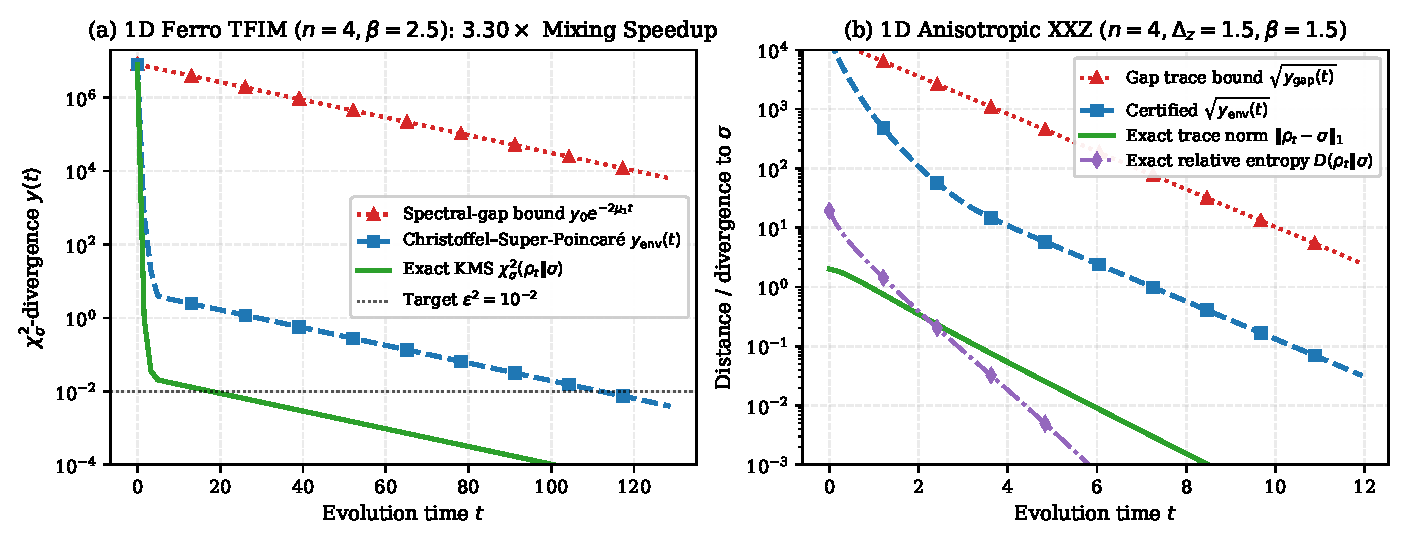
\includegraphics[width=\textwidth]{figures/fig1_1d_kms_trajectories.pdf}
  \caption{\textbf{(a)} Two-stage relaxation of $\chi^2_\sigma(\rho_t\|\sigma)$ on 1D Ferro TFIM ($n=4, \beta=2.5$): the exact Christoffel--Super-Poincar\'e envelope $y_{\mathrm{env}}(t)$ tracks the rapid initial drop and certifies mixing $3.30\times$ faster than $y_{\mathrm{gap}}(t)$. \textbf{(b)} Certified trace-norm and relative-entropy bounds on 1D non-integrable XXZ ($n=4, \Delta_z=1.5, \beta=1.5$).}
  \label{fig:fig1}
\end{figure}

\subsection{Experiment 2: Large-\texorpdfstring{$n$}{n} Pure \texorpdfstring{$L^1 \to L^2$}{L1 -> L2} Scaling and Continuous Phase Diagram}

Figure~\ref{fig:fig2}(a) evaluates the exact integer upper convex hull for the $n$-qubit local depolarizing / commuting Glauber semigroup ($\gamma = 1, \varepsilon = 0.1$) from $n = 10$ up to $n = 1{,}000$: while $T_{\mathrm{gap}}$ grows linearly from $5.77$ to $348.88$, our pure $L^1 \to L^2$ universal Christoffel ($c=3$, valid for all entangled states) and product-state Bloch ($c=1$, valid for all product initial states under product semigroups) bounds grow only poly-logarithmically to $\mathbf{19.69}$ ($\mathbf{17.72\times}$ speedup) and $\mathbf{16.87}$ ($\mathbf{20.68\times}$ speedup) at $n = 1{,}000$, strictly obeying~\eqref{eq:log2n_bound} ($22.82$ analytical cap for $c = 1$). Figure~\ref{fig:fig2}(b) verifies all three closed-form regimes of Theorem~\ref{thm:scaling_phases}(b) ($\alpha \in \{0.5, 1.0, 1.5\}$, $D_2(0) = 50$) against RK45 numerical ODE integration to $< 7.4 \times 10^{-12}$.

\begin{figure}[t]
  \centering
  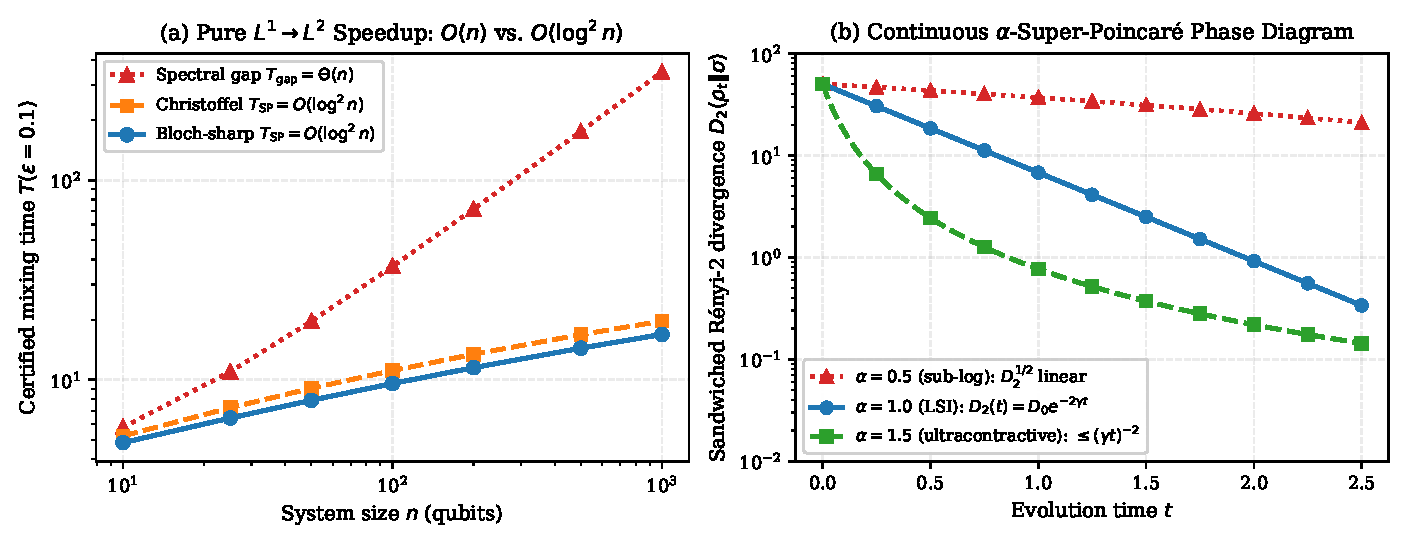
\includegraphics[width=\textwidth]{figures/fig2_scaling_and_alpha_phases.pdf}
  \caption{\textbf{(a)} Pure $L^1 \to L^2$ mixing-time scaling ($n = 10 \to 1{,}000$ qubits, $\varepsilon=0.1$): $T_{\mathrm{gap}} = \Theta(n)$ vs.\ $T_{\mathrm{SP}} = O(\log^2 n)$, reaching $17.7\times$ (universal $c=3$, all states) and $20.7\times$ (product-state $c=1$, product semigroups) speedup at $n = 1{,}000$. \textbf{(b)} Continuous $\alpha$-Super-Poincar\'e phase diagram (Theorem~\ref{thm:scaling_phases}b), contrasting sub-logarithmic ($\alpha=0.5$), double-exponential LSI ($\alpha=1.0$), and finite-time ultracontractive ($\alpha=1.5$) R\'enyi-2 decay.}
  \label{fig:fig2}
\end{figure}

\subsection{Experiments 3--4: Exact-\texorpdfstring{$\Q$}{Q} \texorpdfstring{$\mathrm{LDL}^\top$}{LDLT} Certificates and 2-Tier Sharpness}

Using \texttt{build\_exact\_mixing\_certificate}, we exported and independently verified 6 exact-$\Q$ certificates (Figure~\ref{fig:fig3}b):
\begin{itemize}[leftmargin=1.6em,itemsep=2pt]
  \item \textbf{Linked $\mathrm{LDL}^\top$-verified non-commuting chains (conditioned on input radii $\delta_*^{\Q}$):} On 1D Ferro TFIM ($n=2, \beta=2.0$) and 1D XXZ ($n=2, \beta=2.0$), all 4 active hull tiers are backed by \textbf{14 cryptographically linked exact rational $\mathrm{LDL}^\top$ PSD witnesses} (7 per chain: 4 global operator-order $16 \times 16$ gap matrices + 3 Christoffel $4 \times 4$ norm matrices reconstructed directly from the quantized bundle and tier bounds), certifying $T_{\mathrm{SP}}^{\Q} = 5.980 < T_{\mathrm{gap}}^{\Q} = 7.930$ ($1.33\times$) on TFIM and $T_{\mathrm{SP}}^{\Q} = 5.973 < T_{\mathrm{gap}}^{\Q} = 6.016$ on XXZ strictly over $\Q$ with zero floating-point operations in the verifier (as noted in Sections~\ref{sec:formalization} and~\ref{sec:discussion}, the synthesis script estimates the input Frobenius radii $\delta_*^{\Q}$ against float64 \texttt{eigh(H)} outputs; replacing synthesis with interval-certified eigensolvers upgrades end-to-end provenance from $H$ without altering the verifier).
  \item \textbf{Large-tier exact-$\Q$ convex-hull certificates:} Independently replayed on 1D Ferro TFIM ($n=4, \beta=2.5$, 15 tiers, $3.30\times$), 1D XXZ ($n=4, \beta=1.5$, 19 tiers, $1.57\times$), and $n = 50, 100$ depolarizing chains built strictly in end-to-end exact arbitrary-precision integer arithmetic ($y_0 = 2^{100} - 1$, zero float64 input or truncation above $2^{53}$; $2.17\times, 3.32\times$), while rejecting 15/15 adversarial forgery classes (unlinked witnesses, tampered bounds, \texttt{NaN}/\texttt{Inf}/\texttt{bool} injections, broken knots, missing tier coverage, negative $\mathrm{LDL}^\top$ pivots, and float64 indefinite-matrix bypasses).
  \item \textbf{2-Tier Sharpness (Figure~\ref{fig:fig3}a):} On $\lambda_0 = 0.1, \lambda_1 = 2.0, C_1 = 10, \varepsilon = 0.1$ across $y_0 \in [10^2, 10^8]$, $T_{\mathrm{SP}}$ tracks the exact hitting time $t_{\mathrm{exact}}$ tightly ($T_{\mathrm{SP}} = 39.56$ vs.\ $t_{\mathrm{exact}} = 34.54$, ratio $1.145$, vs.\ $T_{\mathrm{gap}} = 115.13$).
\end{itemize}

\begin{figure}[t]
  \centering
  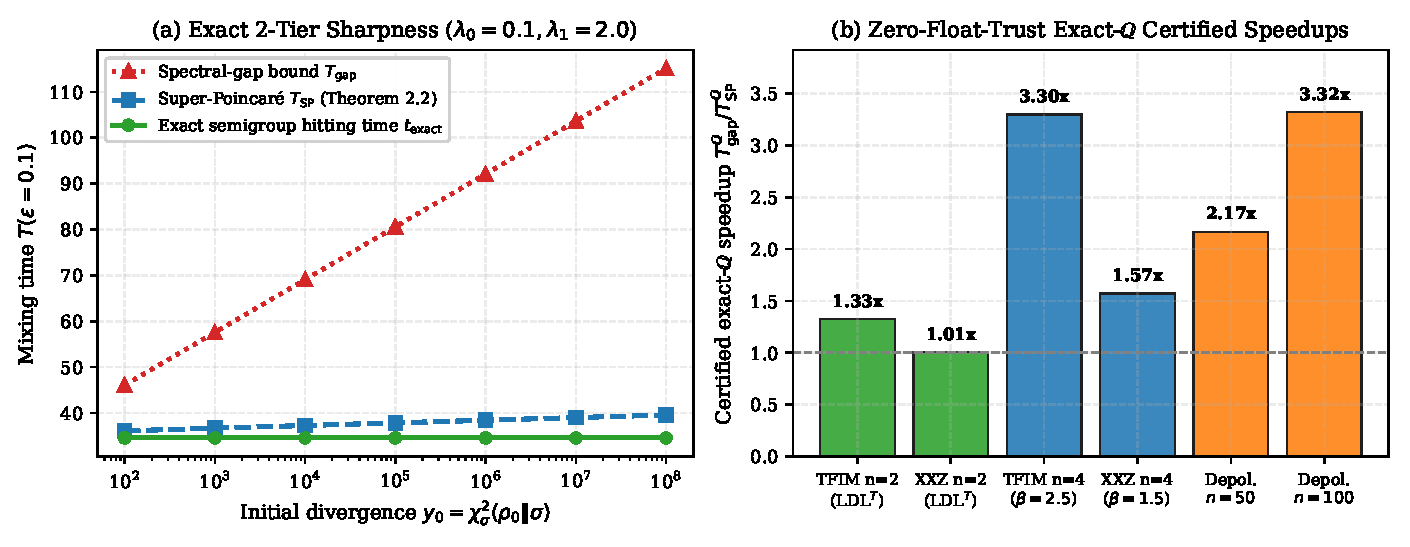
\includegraphics[width=\textwidth]{figures/fig3_sharpness_and_speedups.pdf}
  \caption{\textbf{(a)} Exact 2-tier semigroup sharpness (Theorem~\ref{thm:hull_mixing}c): $T_{\mathrm{SP}}$ tracks $t_{\mathrm{exact}}$ tightly—within ratio $1.045$--$1.145$ across six decades of $y_0$, and within the universal factor-of-2 plus $O(1)$ bound~\eqref{eq:sharp_2tier} for all $y_0$—while $T_{\mathrm{gap}}$ diverges linearly in $\log y_0$. \textbf{(b)} Independently replayed exact-$\Q$ verified speedups across all 6 exported certificates (green bars include 14 verified linked exact-$\Q$ $\mathrm{LDL}^\top$ PSD witnesses on the quantized operator bundle).}
  \label{fig:fig3}
\end{figure}

\section{Discussion, Limitations, and Scope}
\label{sec:discussion}

We have established an exact, non-asymptotic, machine-checked theory of mixing beyond the spectral gap for KMS-symmetric quantum Gibbs samplers via the Quantum Christoffel Operator $\Kchr_V$, exact upper-convex-hull piecewise-logarithmic integration, and exact-$\Q$ global operator-order $\mathrm{LDL}^\top$ certification.

Three honest boundaries frame our results: (i) for \emph{non-invariant} subspaces $V$ (such as Pauli-weight subspaces on interacting Hamiltonians),~\eqref{eq:single_sp} requires the full operator-order Schur constant $\lambda_{\mathrm{op}}(V^\perp) = \sup\{\lambda : -\mathcal{L}^\dagger \succeq \lambda(I - P_V)\}$ rather than the compressed Rayleigh quotient on $V^\perp$ alone—whereas on every $\mathcal{L}^\dagger$-invariant eigenmode subspace $V_r$, both coincide identically with $\mu_{r+1}$ (which is why our exact-$\Q$ certificates and Table~\ref{tab:exp1} use the eigenmode filtration $V_r$); (ii) pure $L^1 \to L^2$ Christoffel projection yields $O(\log^2 n)$ mixing on linear Pauli-weight ladders rather than the optimal $O(\log n)$ achieved by hypercontractivity / quantum LSI, representing a transparent trade-off between completely elementary basis-independent constants and optimal logarithmic exponents; and (iii) exact-$\Q$ dense $\mathrm{LDL}^\top$ certification scales as $O(d^6)$ in Hilbert-space dimension $d = 2^n$ and eliminates eigensolver trust on the quantized operator bundle $(\tilde{M}, \tilde{P}_0, \tilde{P}_k, \tilde{\Kchr}_k)$ given certified Frobenius perturbation radii $\delta_*^{\Q}$ (with our synthesis script estimating $\delta_*^{\Q}$ against float64 \texttt{eigh(H)} outputs), making dense $\mathrm{LDL}^\top$ directly practical for small-to-medium certified subsystems ($n \le 4$) while larger systems feed analytical $\lambda_k$ lower bounds into our exact-$\Q$ convex-hull verifier.

\bibliographystyle{plain}
\bibliography{references}

\end{document}
